% !TeX program = lualatex
% !TeX encoding = utf8

\documentclass[aspectratio=169, 10pt]{beamer}

\usepackage{amsmath}
\usepackage[T1]{fontenc}

\usepackage{lhcb_presentation/package}

\usepackage{units}
\usepackage{graphicx}
\usepackage{booktabs}
\usepackage{ulem}
\usepackage{bm}
\usepackage{comment}
\usepackage{tikz}
\definecolor{brickred}{rgb}{0.85, 0, 0.05}
\errorcontextlines 10000

\title[PV finding with CNNs: Vertexing questions/discussion]{PV finding with CNNs\\{\small Vertexing questions/discussion}}

\author[Fang, Schreiner, Sokoloff]{Rui Fang \and Henry Schreiner \and Mike Sokoloff}
\institute{The University of Cincinnati}
\date{January 16, 2018}

\begin{document}


\begin{frame}
\titlepage
\end{frame}

%%%%%%%%%%%%%%%%%%%%%%%%%%%%%%%%%%%%%%%%%%%%%%%%%%%%%%%%%%%%%%%%%%%%%%%%%%%%%%%

\section{Introduction}

\subsection{Objectives}
\begin{frame}{Objectives}

    \begin{columns}[c]
      \column{.5\textwidth}
      \includegraphics[width=\textwidth, trim=0 0 0 0]{images/LHCbDet.png}
      \begin{block}{Motivation: LHCb upgrade}
        \begin{itemize}
            \item 30 MHz software trigger
            \item 7.6 PVs per event (Poisson distribution)
        \end{itemize}
      \end{block}
    \column{.5\textwidth}

    \begin{block}{Physics}
    \begin{itemize}
        \item Traditional vertexing can be a bottleneck to highly parallel tracking
        \item Vertexing early in trigger algorithms for best performance
        \item Control mistag rate vs. effeciency
    \end{itemize}
    \end{block}

    \begin{block}{Machine learning}
    \begin{itemize}
        \item Sparse 3D data (41M pixels) $\to$ rich 1D data
        \item 1D convolutional neural net
        \item Highly parallelizable, GPU friendly
        \item Opportunity to visualize learning process
    \end{itemize}
    \end{block}

\end{columns}
\end{frame}


\subsection{Tracking in the LHCb upgrade}
\begin{frame}{Tracking in the LHCb upgrade}
  \begin{columns}[c]
    \column{.5\textwidth}
    \begin{block}{The changes}
      \begin{itemize}
          \item 30 MHz software trigger
          \item 7.6 PVs per event (Poisson distribution)
          \item Roughly 5.5 visible PVs per event
      \end{itemize}
    \end{block}
    \begin{block}{The problem}
    \begin{itemize}
    	\item Much higher pileup
    	\item Very little time to do the tracking
    	\item Current algorithms too slow
    \end{itemize}
    \end{block}
    \column{.5\textwidth}
      \begin{center}
    \includegraphics[width=\textwidth, trim=18 0 18 0]{images/LHCbDet.png}
  \end{center}
  \end{columns}

  \vspace{1em}
  \begin{center}
    \textbf{We need to rethink our algorithms from the ground up...}
  \end{center}
\end{frame}


\subsection{A hybrid ML approach}
\begin{frame}{A hybrid ML approach}
\begin{center}
Prototracking $\rightarrow$ Kernel generation $\rightarrow$ CNN to find PVs $\rightarrow$ Informed tracking
\end{center}

\begin{columns}[b]
    \column{.28\textwidth}
    \begin{block}{Prototracking}
    \begin{itemize}
        \item Ultra-simple/fast
        \item Triplets only
        \item Used for kernel only
        \end{itemize}
    \end{block}
    \column{.30\textwidth}
    \begin{block}{Vertexing}
    \begin{itemize}
        \item High efficiency
        \item Low false positive rate
        \item Useful for other reasons
        \end{itemize}
    \end{block}
    \column{.28\textwidth}
    \begin{block}{Tracking}
    \begin{itemize}
        \item Faster (effect TBD)
        \item Uses search windows
        \item Higher efficiency
    \end{itemize}
    \end{block}
\end{columns}
    \begin{block}{Machine learning features (so far)}
        \begin{itemize}
            \item Prototracking converts sparse 3D dataset to feature-rich 1D dataset
            \item Easy and effective visualization due to 1D nature
            \item Can see results with simple unoptimized 2-layer CNN + 1-layer linear
        \end{itemize}
    \end{block}

\vspace{.3em}
\begin{center}
What follows is a proof of principle implementation for finding PVs.
\end{center}
\end{frame}


\subsection{Vertices and tracks}
\begin{frame}{Vertices and tracks}
\begin{columns}[c]
    \column{.5\textwidth}
    \begin{block}{Vertices}
      \begin{itemize}
          \item Events contain $\approx 7$ Primary Vertices (PVs)
          \begin{itemize}
            \item A PV should contain 5+ long tracks
          \end{itemize}
          \item Multiple Secondary Vertices (SVs) per event as well
          \begin{itemize}
            \item A SV should contain 2+ tracks
          \end{itemize}
      \end{itemize}
    \end{block}

    \column{.5\textwidth}
    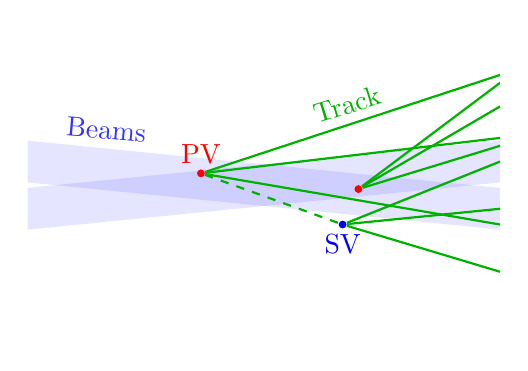
\begin{tikzpicture}
        [beam/.style={line width = 15, opacity=.1, blue, shorten >= -.2cm, shorten <= -.2cm},
        PV/.style={red, circle, fill, inner sep=1pt},
        SV/.style={blue, circle, fill, inner sep=1pt},
        track/.style={green!70!black, thick}]

        \clip [use as bounding box] (-3,-2) rectangle (3,2);
        \clip (-3,-2) rectangle (3,2);

        \node [blue!80!white, rotate=-5] at (-2, .7) {Beams};
        \draw [beam] (-3,.3) -- (3,-.3);
        \draw [beam] (-3,-.3) -- (3,.3);

        \node [PV] (A) at (1.2, -.05) {};
        \node [PV] (B) at (-.8, .15) {};
        \node [red, above] at (B) {PV};

        \draw [track] (A) -- (3,1.3);
        \draw [track] (A) -- (3,1);
        \draw [track] (A) -- (3,.5);

        \draw [track] (B) -- (3,1.4) node [midway, above, rotate=17] {Track};
        \draw [track] (B) -- (3,.6);
        \draw [track] (B) -- (3,-.5);
        \draw [track, dashed] (B) -- (1,-.5);

        \node [SV] (C) at (1,-.5) {};
        \node [blue, below] at (C) {SV};
        \draw [track] (C) -- (3, -.3);
        \draw [track] (C) -- (3, .3);
        \draw [track] (C) -- (3, -1.1);
    \end{tikzpicture}
  \end{columns}

  \begin{block}{}
  \begin{itemize}
      \item We are developing a way to find PVs and SVs using hit triplets
      \item This will enable an iterative tracking algorithm
  \end{itemize}
  \end{block}
\end{frame}


%%%%%%%%%%%%%%%%%%%%%%%%%%%%%%%%%%%%%%%%%%%%%%%%%%%%%%%%%%%%%%%%%%%%%%%%%%%%%%%

\section{Design}

\subsection{Kernel generation}
\begin{frame}{Kernel generation}
  \begin{columns}[c]
    \column{.54\textwidth}

        \begin{block}{Tracking procedure}
        \begin{itemize}
            \item Hits lie on the 26 planes
            \item For simplicity, only 3 tracks shown
            \uncover<2->{%
            \item Make a 3D grid of voxels (2D shown)
            \item \textcolor{lhcbRed}{Note: only $z$ will be fully calculated and stored}
            }
            \uncover<3->{%
            \item Tracking (full or partial)
            }
            \uncover<4->{%
            \item Fill in each voxel center with gaussian PDF
            }
            \uncover<5->{%
            \item PDF for each (proto)track is combined
            }
            \uncover<6->{%
            \item Stores $z$ histogram with maximum KDE value
            }
        \end{itemize}
        \end{block}

    \column{.46\textwidth}
    \begin{tikzpicture}
        [hit/.style={inner sep=2pt, fill, circle, black!80!red},
        simitrack/.style={shorten >= -6cm, shorten <= -6cm, opacity=.2, line width=.1cm,
            preaction={draw, line width=.3cm, opacity=.2},
            preaction={draw, line width=.5cm, opacity=.2}},
        bluesimitrack/.style={thick, blue,
            preaction={shorten >= -6cm, shorten <= -6cm, draw, opacity=.2, line width=.1cm,
                preaction={draw, blue, line width=.3cm, opacity=.2},
                preaction={draw, blue, line width=.5cm, opacity=.2}}}
        ]

        \node at (2,-3) [below] {$z$ axis (along the beam)};
        \node at (-1, 0) [left] {$x$};

        \clip (-1,-3) rectangle (5,3);

        \begin{scope}[xscale=.65, xshift=-.6cm]

        % def f(name, slope, factor):
        %     v = np.arange(1,9)
        %     vv = (v-.5)*slope + .05*np.sin(v*factor)
        %     q = np.linspace(.5, 8, 400)
        %     qq = (q-.5)*slope + .05*np.sin(q*factor)
        %     print(f'% {name} slope={slope} factor={factor}')
        %     for a,b in zip(v,vv):
        %         print(f'\coordinate ({name}{a}) at ({a}, {b:.3});')
        %     print()
        %     return q, qq, v, vv


        % (v-.5)*slope + .05*np.sin(v*factor)
        % A slope=0.4 factor=-5
        \coordinate (A7) at (1, 0.248);
        \coordinate (A6) at (2, 0.627);
        \coordinate (A5) at (3, 0.967);
        \coordinate (A4) at (4, 1.35);
        \coordinate (A3) at (5, 1.81);
        \coordinate (A2) at (6, 2.25);
        \coordinate (A1) at (7, 2.62);

        % B slope=0.06 factor=6
        \coordinate (B8) at (1, 0.016);
        \coordinate (B7) at (2, 0.0632);
        \coordinate (B6) at (3, 0.112);
        \coordinate (B5) at (4, 0.165);
        \coordinate (B4) at (5, 0.221);
        \coordinate (B3) at (6, 0.28);
        \coordinate (B2) at (7, 0.344);
        \coordinate (B1) at (8, 0.412);

        % C slope=-0.35 factor=7
        \coordinate (C7) at (1, -0.142);
        \coordinate (C6) at (2, -0.475);
        \coordinate (C5) at (3, -0.833);
        \coordinate (C4) at (4, -1.21);
        \coordinate (C3) at (5, -1.6);
        \coordinate (C2) at (6, -1.97);
        \coordinate (C1) at (7, -2.32);

        \only<1>{%
        \foreach \x in {0,...,9}{%
            \draw [ultra thick, yellow!80!black] (\x, -3) -- (\x,3);
        }
        }

        \only<2>{%
        \foreach \x in {0,...,9}{%
            \draw [ultra thick, yellow!80!black, opacity=.5] (\x, -3) -- (\x,3);
        }
        }
        \end{scope}

        \only<2->{%
        \draw[step=.35, gray, very thin, use as bounding box] (-1,-3) grid (5,3);
        }

        \only<3>{%
            \draw [bluesimitrack] (A5) -- (A7) ;
        } \only<4->{%
            \draw [simitrack] (A5) -- (A7) ;
        }

        \only<4>{%
            \draw [bluesimitrack] (B6) -- (B8) ;
        } \only<5->{%
            \draw [simitrack] (B6) -- (B8) ;
        }

        \only<5>{%
            \draw [bluesimitrack] (C5) -- (C7) ;
        } \only<6->{%
            \draw [simitrack] (C5) -- (C7) ;
        }

        \draw [fill,green!60!black] (0,0) circle (.065) node [left] {PV};

        \only<0-2>{%
        \node [hit] at (A1) {};
        \node [hit] at (A2) {};
        \node [hit] at (A3) {};
        \node [hit] at (A4) {};
        }\only<3->{%
        \node [hit, red] at (A1) {};
        \node [hit, red] at (A2) {};
        \node [hit, red] at (A3) {};
        \node [hit, red] at (A4) {};
        }

        \only<0-2>{%
        \node [hit] at (A5) {};
        \node [hit] at (A6) {};
        \node [hit] at (A7) {};
        } \only<3>{%
        \node [hit, blue] at (A5) {};
        \node [hit, blue] at (A6) {};
        \node [hit, blue] at (A7) {};
        } \only<4->{%
        \node [hit, red] at (A5) {};
        \node [hit, red] at (A6) {};
        \node [hit, red] at (A7) {};
        }

        \only<0-3>{%
        \node [hit] at (B1) {};
        \node [hit] at (B2) {};
        \node [hit] at (B3) {};
        \node [hit] at (B4) {};
        \node [hit] at (B5) {};
        } \only<4->{%
        \node [hit, red] at (B1) {};
        \node [hit, red] at (B2) {};
        \node [hit, red] at (B3) {};
        \node [hit, red] at (B4) {};
        \node [hit, red] at (B5) {};
        }

        \only<0-3>{%
        \node [hit] at (B6) {};
        \node [hit] at (B7) {};
        \node [hit] at (B8) {};
        } \only<4>{%
        \node [hit, blue] at (B6) {};
        \node [hit, blue] at (B7) {};
        \node [hit, blue] at (B8) {};
        }\only<5->{%
        \node [hit, red] at (B6) {};
        \node [hit, red] at (B7) {};
        \node [hit, red] at (B8) {};
        }

        \only<0-4>{%
        \node [hit] at (C1) {};
        \node [hit] at (C2) {};
        \node [hit] at (C3) {};
        \node [hit] at (C4) {};
        } \only<5->{%
        \node [hit, red] at (C1) {};
        \node [hit, red] at (C2) {};
        \node [hit, red] at (C3) {};
        \node [hit, red] at (C4) {};
        }

        \only<0-4>{%
        \node [hit] at (C5) {};
        \node [hit] at (C6) {};
        \node [hit] at (C7) {};
        } \only<5>{%
        \node [hit, blue] at (C5) {};
        \node [hit, blue] at (C6) {};
        \node [hit, blue] at (C7) {};
        } \only<6->{%
        \node [hit, red] at (C5) {};
        \node [hit, red] at (C6) {};
        \node [hit, red] at (C7) {};
        }

    \end{tikzpicture}

    \end{columns}
\end{frame}


\subsection{Example of z KDE histogram}
\begin{frame}{Example of z KDE histogram}
\begin{center}
    \includegraphics[width=\textwidth, trim=50 30 50 30]{images/kernel_and_pvs.pdf}
\end{center}
\begin{columns}[b]
    \column{.55\textwidth}

    \textcolor{lhcbRed}{Note: All events from toy detector simulation}

    \begin{block}{Human learning}
    \begin{itemize}
        \item Peaks generally correspond to PVs and SVs
    \end{itemize}
    \end{block}

    \column{.45\textwidth}
    \begin{block}{Challenges}
    \begin{itemize}
        \item Vertex may be offset from peak
        \item Vertices interact
    \end{itemize}
    \end{block}
\end{columns}
\end{frame}


\subsection{Target distribution}
\begin{frame}{Target distribution}
\begin{columns}[c]
    \column{.5\textwidth}
    \begin{block}{Build target distribution}
      \begin{itemize}
          \item real PV position as the mean of Gaussian distribution
          \item $\sigma $(standard deviation) is 100 $\mu$m
          \item calculate the cdf of each bin around of the mean, within $\pm$ 3 bins ($\pm$ 300 $\mu$m )
      \end{itemize}
    \end{block}
    \begin{center}
            \includegraphics[width=1\textwidth,height=0.45\textwidth,trim=18 0 18 0]{images/T_1_12.png}

        \end{center}
    \column{.5\textwidth}
      \begin{center}
    \includegraphics[width=1\textwidth,height=0.45\textwidth, trim=18 0 18 0]{images/T_2_12.png}

    \includegraphics[width=1\textwidth,height=0.45\textwidth, trim=18 0 18 0]{images/T_2_25.png}
  \end{center}
  \end{columns}
\end{frame}


\subsection{Preliminary study}
\begin{frame}{Preliminary study}
\begin{columns}[c]
    \column{.5\textwidth}
    \begin{block}{Preliminary study}
      \begin{itemize}
          \item 2, 3, and 4 convolutional layers
          \item Symmetric cost function to be described
          \item Discovered ``low multiplicity'' PVs are counted as false positives
      \end{itemize}
    \end{block}
    \column{.5\textwidth}
    \begin{block}{Current work}
      \begin{itemize}
          \item Add masking to not count discovered ``low multiplicity'' as false positives
          \item Asymmetric cost function to control trade-offs between efficiency  and false positive rates
      \end{itemize}
    \end{block}
  \end{columns}
\end{frame}



\subsection{Neural network architecture}
\begin{frame}{Neural network architecture with two convolutional layers}
    \begin{center}
      \includegraphics[width=0.75\linewidth, trim=0 30 0 0]{images/CNN_2.png}
   \end{center}
   \begin{itemize}
       \item Activation function for hidden layers: Leaky ReLu
       \item Activation function for output layer: Sigmoid
   \end{itemize}
\end{frame}

\begin{frame}{Activation function}
   \begin{columns}[c]
   % TODO: Swap
        \column{.5\textwidth}
        \begin{center}
            \includegraphics[width=0.8\textwidth]{images/LeakyRelu.png}

            Activation function for hidden layers
        \end{center}

        \column{.5\textwidth}
        \begin{center}
            \includegraphics[width=0.8\textwidth]{images/Sigmoid.png}

            Activation function for output layer
        \end{center}
  \end{columns}
\end{frame}


\subsection{Cost function}
\begin{frame}{Cost function}
    \begin{block}{Approach}
      \begin{itemize}
         \item
            Should be similar to Cross-Entropy for $ y \to 0 $,
           $ y \to 1 $;
             $ \color{brickred} \textrm{cost} = - \left (y \ln \hat{y} + (1-y) \ln (1 - \hat{y}) \right )  $
         \item
          Should be symmetric with respect to  $ r = ( \hat y/y  )$ \& $ 1/r $
     \end{itemize}
     \vspace{-.3cm}

     \[
     r_i \equiv (\hat{y_i} + \epsilon)/ (y_i + \epsilon)
     \quad
     z_i \equiv \frac{2 \, r_i }{r_i + 1/r_i}
     \]
    \end{block}

  \begin{columns}[c]
    \column{0.33\textwidth}
    \centering
    \includegraphics[width=\textwidth]{images/AltCostPlot_181015.png}
    \column{0.33\textwidth}
    \centering
    \includegraphics[width=\textwidth]{images/AltCostPlot_181015_linearA.png}
    \column{0.33\textwidth}
    \centering
    \includegraphics[width=\textwidth]{images/AltCostPlot_181015_linear.png}
    \end{columns}
\end{frame}


%%%%%%%%%%%%%%%%%%%%%%%%%%%%%%%%%%%%%%%%%%%%%%%%%%%%%%%%%%%%%%%%%%%%%%%%%%%%%%%

\section{Results}

\subsection{Cost plot}
\begin{frame}{Cost, efficiency, and false positive rate: 2 convolutionial layers}
   \centering
   \includegraphics[width=0.45\linewidth]{images/CNN_2Layer_Cost.png}
   \includegraphics[width=0.45\linewidth]{images/CNN_2Layer_FalsePositive.png}

\end{frame}

\begin{frame}{Cost, efficiency, and false positive rate: 3 convolutionial layers}
   \centering
   \includegraphics[width=0.45\linewidth]{images/CNN_3Layer_Cost.png}
   \includegraphics[width=0.45\linewidth]{images/CNN_3Layer_FalsePositive.png}

\end{frame}


\subsection{Prediction plots}
\begin{frame}{Compare predictions with targets: Examples}
  \begin{columns}[c]
    \column{.5\textwidth}
        \begin{center}
           \includegraphics[width=1\textwidth, trim=60 40 60 20]{images/07Jan19_AltCNN4Layer_D35_sp_30.pdf}

           \textbf{\color{lhcbBlue}\large PV found example}
       \end{center}
   \column{.5\textwidth}
       \begin{center}
           \includegraphics[width=1\textwidth, trim=60 40 60 20]{images/07Jan19_AltCNN4Layer_D35_sp_32.pdf}

           \textbf{\color{lhcbBlue}\large PV found example}
       \end{center}
  \end{columns}
\end{frame}

\begin{frame}{Compare predictions with targets: When it works}
  \begin{columns}[c]
    \column{.5\textwidth}
        \begin{center}
           \includegraphics[width=1\textwidth, trim=60 40 60 20]{images/07Jan19_AltCNN4Layer_D35_sp_02.pdf}

           \textbf{\color{lhcbBlue}\large PV found example}
       \end{center}
   \column{.5\textwidth}
       \begin{center}
           \includegraphics[width=1\textwidth, trim=60 40 60 20]{images/07Jan19_AltCNN4Layer_D35_sp_01.pdf}

           \textbf{\color{lhcbBlue}\large Masked (<5 tracks) example}
       \end{center}
  \end{columns}
\end{frame}


\begin{frame}{Compare predictions with targets: When it fails}
  \begin{columns}[c]
    \column{.5\textwidth}
        \begin{center}
           \includegraphics[width=1\textwidth, trim=60 40 60 20]{images/07Jan19_AltCNN4Layer_D35_sp_10.pdf}

           \textbf{\color{lhcbRed}\large False Positive example}
        \end{center}
    \column{.5\textwidth}
        \begin{center}
           \includegraphics[width=1\textwidth, trim=60 40 60 20]{images/07Jan19_AltCNN4Layer_D35_sp_15.pdf}

           \textbf{\color{lhcbRed}\large PV not found example}
       \end{center}
  \end{columns}
\end{frame}


\subsection{Quantitative results}
\begin{frame}{Efficiencies and false positive rates}
\begin{columns}
\column{.5\textwidth}
\includegraphics[width=\textwidth]{images/EffVsFP.pdf}
\column{.5\textwidth}
\includegraphics[width=\textwidth]{images/EffVsFP_semilog.pdf}
\end{columns}

  \begin{columns}
      \column{.5\textwidth}
  \begin{block}{Search for PVs}
    \begin{itemize}
    	\item Search $ \pm 5 $ bins ($ \pm 500 \mu $m) around a true PV
    	\item At least 3 bins with predicted probability
    	   $ > 1\% $ and
    	   integrated probability $ > 20\%$.
    \end{itemize}
    \end{block}

    \column{.5\textwidth}
    \begin{block}{Tunable efficiency vs.\ FP}
    \begin{itemize}
        \item The asymmetry parameter controls efficiency vs.\ FP
    \end{itemize}
  \end{block}
\end{columns}
\end{frame}


\subsection{Asymmetric loss}
\begin{frame}{Asymmetric loss}
    \centerline{
        \begin{minipage}[t]{1.1\textwidth}
            \includegraphics[width=.33\textwidth, clip, trim=10 0 40 0]{images/AltCostPlot_181015}
            \includegraphics[width=.33\textwidth, clip, trim=10 0 40 0]{images/AltCostPlot_181015_linear}
            \includegraphics[width=.33\textwidth, clip, trim=10 0 40 0]{images/AltCostPlot_181015_linearA}
        \end{minipage}
    }
\end{frame}


\subsection {New quantitative results}
\begin{frame}{Efficiencies and false positive rates, cont.}
\begin{table}[]
\centering
    {\Large With masking} \\
    \vspace{.5em}
\begin{tabular}{ccccc}
    Layers (Conv. + FC Linear) & 3 + 1 & 4 + 1 & 4 + 1  & 5 + 0\\[.3em]
    Sym or asym loss      & Sym          & Sym             & Asym & Asym     \\ [0.9em]
    $ \epsilon \textrm{(Efficiency)} = \frac{\mbox{TP}}{\mbox{TP} + \mbox{FN}} $ &  $ \approx 80\% $  & $ \approx 82\% $ & $ \approx 92\% $ & $ \approx 93.6\% $ \\ [0.9em]
    $ \textrm{FP rate} = \frac{\mbox{FP}}{\mbox{number of events}} $ &  $\approx 0.03  $  & $\approx 0.03  $ & $ \approx 0.18 $ & $ \approx 0.22\ (4\%) $ \\
 \end{tabular}
\end{table}

Note: For 10+ long tracks, the efficiency is around 97\%-98\% for the larger networks.
\end{frame}


%%%%%%%%%%%%%%%%%%%%%%%%%%%%%%%%%%%%%%%%%%%%%%%%%%%%%%%%%%%%%%%%%%%%%%%%%%%%%%%


\section{Future plans}

\subsection{Future plans}
\begin{frame}{Conclusions and plans}
    \begin{tikzpicture}[overlay, remember picture]
        \node at (current page.center) {\includegraphics[width=14.7cm]{images/effntracks_bg.pdf}};
    \end{tikzpicture}
\begin{columns}
\column{.25\textwidth}
\column{.65\textwidth}
\setstretch{0.92}
\vskip -1.75em
    \begin{itemize}
    \setlength\itemsep{0.25em}
        \item [\textcolor{lhcbRed}{\textbullet}] \color{lhcbRed}
          Proof-of-Principle established:
          \color{lhcbBlue}
          a hybrid ML algorithm using a 1-dimensional KDE processed by a 5-layer CNN finds primary vertices with efficiencies and false positive rates similar to traditional algorithms.
        \item [\textcolor{lhcbRed}{\textbullet}] \color{lhcbRed} Efficiency is tunable; \color{lhcbBlue} increasing the efficiency also increases the false positive rate.
        \item [\textcolor{lhcbRed}{\textbullet}] \color{lhcbRed} Adding information
        should improve performance.
        \color{lhcbBlue}
        \begin{itemize}
            \item [\textcolor{lhcbBlue}
            {\textbullet} \color{lhcbBlue}] \color{lhcbBlue}
            can add KDE (x,y) information to algorithm
            \item [\color{lhcbBlue}{\textbullet} \color{lhcbBlue}]
            \color{lhcbBlue} can associate tracks to PV candidates, then iterate.
        \end{itemize}
        \item [\textcolor{lhcbRed}{\textbullet}] \color{lhcbRed} Next steps:
        \color{lhcbBlue}
        train with full LHCb MC and deploy inference engine in LHCb Hlt1 framework.
        \item [\textcolor{lhcbRed}{\textbullet}] \color{lhcbRed} Beyond LHCb
        \begin{itemize}
            \item [\color{lhcbBlue} {\textbullet}] \color{lhcbBlue}
                approach might work for ATLAS and CMS (in 2D?);
            \item [\color{lhcbBlue} {\textbullet}] \color{lhcbBlue} algorithm is an interesting ML laboratory.
        \end{itemize}
    \end{itemize}
\column{.1\textwidth}
\end{columns}
\end{frame}


\subsection{Questions}
\begin{frame}{Questions for ATLAS and CMS}
    \begin{itemize}
      \item
          Beam width ($x$, $y$): $\unit[40]{\mu m}$ for LHCb; what are the widths for ATLAS and CMS?
      \item
          Transverse resolution: $\unit[5\textup{--}15]{\mu m}$ for LHCb depending on number of tracks; what is it for ATLAS and CMS?
      \item
          Longitudinal resolution: $\unit[40\textup{--}100]{\mu m}$ for LHCb depending on number of tracks; what is it for ATLAS and CMS?
      \item
          Cleaning up prototracks based on IP could simplify kernel
      \item
          Can prototracking be done in the ATLAS and CMS triggers?
    \end{itemize}
\end{frame}


%%%%%%%%%%%%%%%%%%%%%%%%%%%%%%%%%%%%%%%%%%%%%%%%%%%%%%%%%%%%%%%%%%%%%%%%%%%%%%%

\backupbegin
\section{Backup}

\subsection{Predictions with targets}
\begin{frame}{Compare predictions with targets (3 convolutional layers)}
  \begin{columns}[c]
    \column{.5\textwidth}
        \begin{center}
            \includegraphics[width=1\textwidth,height=0.45\textwidth, trim=18 0 18 0]{images/120000_3layer_04.pdf}

            \includegraphics[width=1\textwidth, height=0.45\textwidth,trim=18 0 18 0]{images/120000_3layer_05.pdf}

        \end{center}
    \column{.5\textwidth}
        \begin{center}
           \includegraphics[width=1\textwidth, height=0.45\textwidth, trim=18 0 18 0]{images/120000_3layer_06.pdf}

           \includegraphics[width=1\textwidth, height=0.45\textwidth, trim=18 0 18 0]{images/120000_3layer_07.pdf}
       \end{center}
  \end{columns}
\end{frame}

\begin{frame}{Compare predictions with targets (3 convolutional layers)}
  \begin{columns}[c]
    \column{.5\textwidth}
        \begin{center}
            \includegraphics[width=1\textwidth,height=0.45\textwidth, trim=18 0 18 0]{images/120000_3layer_08.pdf}

            \includegraphics[width=1\textwidth, height=0.45\textwidth,trim=18 0 18 0]{images/120000_3layer_09.pdf}

        \end{center}
    \column{.5\textwidth}
        \begin{center}
           \includegraphics[width=1\textwidth, height=0.45\textwidth, trim=18 0 18 0]{images/120000_3layer_10.pdf}

           \includegraphics[width=1\textwidth, height=0.45\textwidth, trim=18 0 18 0]{images/120000_3layer_11.pdf}
       \end{center}
  \end{columns}
\end{frame}


\subsection{More predictions with targets}

\begin{frame}{More predictions with targets (3 CVN layers)}
  \begin{columns}[c]
    \column{.5\textwidth}
        \begin{center}
            \includegraphics[width=1\textwidth,height=0.45\textwidth, trim=18 0 18 0]{images/120000_3layer_16.pdf}

            \includegraphics[width=1\textwidth, height=0.45\textwidth,trim=18 0 18 0]{images/120000_3layer_17.pdf}

        \end{center}
    \column{.5\textwidth}
        \begin{center}
           \includegraphics[width=1\textwidth, height=0.45\textwidth, trim=18 0 18 0]{images/120000_3layer_18.pdf}

           \includegraphics[width=1\textwidth, height=0.45\textwidth, trim=18 0 18 0]{images/120000_3layer_19.pdf}
       \end{center}
  \end{columns}
\end{frame}

\begin{frame}{More Predictions with Targets (3 CVN layers)}
  \begin{columns}[c]
    \column{.5\textwidth}
        \begin{center}
            \includegraphics[width=1\textwidth,height=0.45\textwidth, trim=18 0 18 0]{images/120000_3layer_20.pdf}

            \includegraphics[width=1\textwidth, height=0.45\textwidth,trim=18 0 18 0]{images/120000_3layer_21.pdf}

        \end{center}
    \column{.5\textwidth}
        \begin{center}
           \includegraphics[width=1\textwidth, height=0.45\textwidth, trim=18 0 18 0]{images/120000_3layer_22.pdf}

           \includegraphics[width=1\textwidth, height=0.45\textwidth, trim=18 0 18 0]{images/120000_3layer_23.pdf}
       \end{center}
  \end{columns}
\end{frame}

\begin{frame}{More Predictions with Targets (3 CVN layers)}
  \begin{columns}[c]
    \column{.5\textwidth}
        \begin{center}
            \includegraphics[width=1\textwidth,height=0.45\textwidth, trim=18 0 18 0]{images/120000_3layer_24.pdf}

            \includegraphics[width=1\textwidth, height=0.45\textwidth,trim=18 0 18 0]{images/120000_3layer_25.pdf}

        \end{center}
    \column{.5\textwidth}
        \begin{center}
           \includegraphics[width=1\textwidth, height=0.45\textwidth, trim=18 0 18 0]{images/120000_3layer_26.pdf}

           \includegraphics[width=1\textwidth, height=0.45\textwidth, trim=18 0 18 0]{images/120000_3layer_27.pdf}
       \end{center}
  \end{columns}
\end{frame}

\begin{frame}{More Predictions with Targets (3 CVN layers)}
  \begin{columns}[c]
    \column{.5\textwidth}
        \begin{center}
            \includegraphics[width=1\textwidth,height=0.45\textwidth, trim=18 0 18 0]{images/120000_3layer_28.pdf}

            \includegraphics[width=1\textwidth, height=0.45\textwidth,trim=18 0 18 0]{images/120000_3layer_29.pdf}

        \end{center}
    \column{.5\textwidth}
        \begin{center}
           \includegraphics[width=1\textwidth, height=0.45\textwidth, trim=18 0 18 0]{images/120000_3layer_30.pdf}

           \includegraphics[width=1\textwidth, height=0.45\textwidth, trim=18 0 18 0]{images/120000_3layer_31.pdf}
       \end{center}
  \end{columns}
\end{frame}

\begin{frame}{More Predictions with Targets (3 CVN layers)}
  \begin{columns}[c]
    \column{.5\textwidth}
        \begin{center}
            \includegraphics[width=1\textwidth,height=0.45\textwidth, trim=18 0 18 0]{images/120000_3layer_32.pdf}

            \includegraphics[width=1\textwidth, height=0.45\textwidth,trim=18 0 18 0]{images/120000_3layer_33.pdf}

        \end{center}
    \column{.5\textwidth}
        \begin{center}
           \includegraphics[width=1\textwidth, height=0.45\textwidth, trim=18 0 18 0]{images/120000_3layer_34.pdf}

           \includegraphics[width=1\textwidth, height=0.45\textwidth, trim=18 0 18 0]{images/120000_3layer_35.pdf}
       \end{center}
  \end{columns}
\end{frame}

\begin{frame}{More Predictions with Targets (3 CVN layers)}
  \begin{columns}[c]
    \column{.5\textwidth}
        \begin{center}
            \includegraphics[width=1\textwidth,height=0.45\textwidth, trim=18 0 18 0]{images/120000_3layer_36.pdf}

            \includegraphics[width=1\textwidth, height=0.45\textwidth,trim=18 0 18 0]{images/120000_3layer_37.pdf}

        \end{center}
    \column{.5\textwidth}
        \begin{center}
           \includegraphics[width=1\textwidth, height=0.45\textwidth, trim=18 0 18 0]{images/120000_3layer_38.pdf}

           \includegraphics[width=1\textwidth, height=0.45\textwidth, trim=18 0 18 0]{images/120000_3layer_39.pdf}
       \end{center}
  \end{columns}
\end{frame}

\begin{frame}{More Predictions with Targets (3 CVN layers)}
  \begin{columns}[c]
    \column{.5\textwidth}
        \begin{center}
            \includegraphics[width=1\textwidth,height=0.45\textwidth, trim=18 0 18 0]{images/120000_3layer_40.pdf}

            \includegraphics[width=1\textwidth, height=0.45\textwidth,trim=18 0 18 0]{images/120000_3layer_41.pdf}

        \end{center}
    \column{.5\textwidth}
        \begin{center}
           \includegraphics[width=1\textwidth, height=0.45\textwidth, trim=18 0 18 0]{images/120000_3layer_42.pdf}

           \includegraphics[width=1\textwidth, height=0.45\textwidth, trim=18 0 18 0]{images/120000_3layer_43.pdf}
       \end{center}
  \end{columns}
\end{frame}

\begin{frame}{More Predictions with Targets (3 CVN layers)}
  \begin{columns}[c]
    \column{.5\textwidth}
        \begin{center}
            \includegraphics[width=1\textwidth,height=0.45\textwidth, trim=18 0 18 0]{images/120000_3layer_45.pdf}

            \includegraphics[width=1\textwidth, height=0.45\textwidth,trim=18 0 18 0]{images/120000_3layer_46.pdf}

        \end{center}
    \column{.5\textwidth}
        \begin{center}
           \includegraphics[width=1\textwidth, height=0.45\textwidth, trim=18 0 18 0]{images/120000_3layer_47.pdf}

           \includegraphics[width=1\textwidth, height=0.45\textwidth, trim=18 0 18 0]{images/120000_3layer_48.pdf}
       \end{center}
  \end{columns}
\end{frame}

\begin{frame}{More Predictions with Targets (3 CVN layers)}
  \begin{columns}[c]
    \column{.5\textwidth}
        \begin{center}
            \includegraphics[width=1\textwidth,height=0.45\textwidth, trim=18 0 18 0]{images/120000_3layer_49.pdf}

            \includegraphics[width=1\textwidth, height=0.45\textwidth,trim=18 0 18 0]{images/120000_3layer_50.pdf}

        \end{center}
    \column{.5\textwidth}
        \begin{center}
           \includegraphics[width=1\textwidth, height=0.45\textwidth, trim=18 0 18 0]{images/120000_3layer_51.pdf}

           \includegraphics[width=1\textwidth, height=0.45\textwidth, trim=18 0 18 0]{images/120000_3layer_52.pdf}
       \end{center}
  \end{columns}
\end{frame}

\begin{frame}{More Predictions with Targets (3 CVN layers)}
  \begin{columns}[c]
    \column{.5\textwidth}
        \begin{center}
            \includegraphics[width=1\textwidth,height=0.45\textwidth, trim=18 0 18 0]{images/120000_3layer_53.pdf}

            \includegraphics[width=1\textwidth, height=0.45\textwidth,trim=18 0 18 0]{images/120000_3layer_54.pdf}

        \end{center}
    \column{.5\textwidth}
        \begin{center}
           \includegraphics[width=1\textwidth, height=0.45\textwidth, trim=18 0 18 0]{images/120000_3layer_55.pdf}

           \includegraphics[width=1\textwidth, height=0.45\textwidth, trim=18 0 18 0]{images/120000_3layer_56.pdf}
       \end{center}
  \end{columns}
\end{frame}


\subsection{The VELO}
\begin{frame}{The VELO}
  \begin{columns}[c]
    \column{.6\textwidth}
    \begin{block}{Tracks}
      \begin{itemize}
          \item Originate from vertices (not shown)
          \item Hits originate from tracks
          \item We only know the true track in simulation
          \item Nearly straight, but tracks may scatter in material
      \end{itemize}
    \end{block}
    \begin{block}{The VELO}
      \begin{itemize}
          \item A set of 26 planes that detect tracks
          \item Tracks should hit one or more pixels per plane
          \item Sparse 3D dataset (41M pixels)
      \end{itemize}
    \end{block}
    \column{.4\textwidth}
    \centering
    \includegraphics[width=\textwidth, trim=200 0 100 0]{images/Intersections.png}
  \end{columns}
\end{frame}


\backupend


\end{document}
